%% BioMed_Central_Tex_Template_v1.06
%%                                      %
%  bmc_article.tex            ver: 1.06 %
%                                       %

%%IMPORTANT: do not delete the first line of this template
%%It must be present to enable the BMC Submission system to 
%%recognise this template!!

%%%%%%%%%%%%%%%%%%%%%%%%%%%%%%%%%%%%%%%%%
%%                                     %%
%%  LaTeX template for BioMed Central  %%
%%     journal article submissions     %%
%%                                     %%
%%         <14 August 2007>            %%
%%                                     %%
%%                                     %%
%% Uses:                               %%
%% cite.sty, url.sty, bmc_article.cls  %%
%% ifthen.sty. multicol.sty		   %%
%%				      	   %%
%%                                     %%
%%%%%%%%%%%%%%%%%%%%%%%%%%%%%%%%%%%%%%%%%


%%%%%%%%%%%%%%%%%%%%%%%%%%%%%%%%%%%%%%%%%%%%%%%%%%%%%%%%%%%%%%%%%%%%%
%%                                                                 %%	
%% For instructions on how to fill out this Tex template           %%
%% document please refer to Readme.pdf and the instructions for    %%
%% authors page on the biomed central website                      %%
%% http://www.biomedcentral.com/info/authors/                      %%
%%                                                                 %%
%% Please do not use \input{...} to include other tex files.       %%
%% Submit your LaTeX manuscript as one .tex document.              %%
%%                                                                 %%
%% All additional figures and files should be attached             %%
%% separately and not embedded in the \TeX\ document itself.       %%
%%                                                                 %%
%% BioMed Central currently use the MikTex distribution of         %%
%% TeX for Windows) of TeX and LaTeX.  This is available from      %%
%% http://www.miktex.org                                           %%
%%                                                                 %%
%%%%%%%%%%%%%%%%%%%%%%%%%%%%%%%%%%%%%%%%%%%%%%%%%%%%%%%%%%%%%%%%%%%%%


\NeedsTeXFormat{LaTeX2e}[1995/12/01]
%\RequirePackage{fixltx2e}
\documentclass[10pt]{bmc_article}    

% Load packages
\usepackage{cite} % Make references as [1-4], not [1,2,3,4]
\usepackage{url}  % Formatting web addresses  
\usepackage{ifthen}  % Conditional 
\usepackage{multicol}   %Columns
\usepackage[utf8x]{inputenc} 
\usepackage[pdftex]{graphicx}
\usepackage{verbatim} 
\usepackage{booktabs}
\usepackage{placeins}
\usepackage{xr}
\usepackage{hyperref}
\externaldocument[SI-]{SI}

\usepackage{amsmath}
\usepackage{tensor}

%\usepackage[applemac]{inputenc} %applemac support if unicode package fails
%\usepackage[latin1]{inputenc} %UNIX support if unicode package fails
\urlstyle{rm}
 
 
%%%%%%%%%%%%%%%%%%%%%%%%%%%%%%%%%%%%%%%%%%%%%%%%%	
%%                                             %%
%%  If you wish to display your graphics for   %%
%%  your own use using includegraphic or       %%
%%  includegraphics, then comment out the      %%
%%  following two lines of code.               %%   
%%  NB: These line *must* be included when     %%
%%  submitting to BMC.                         %% 
%%  All figure files must be submitted as      %%
%%  separate graphics through the BMC          %%
%%  submission process, not included in the    %% 
%%  submitted article.                         %% 
%%                                             %%
%%%%%%%%%%%%%%%%%%%%%%%%%%%%%%%%%%%%%%%%%%%%%%%%%                     
%\def\includegraphic{}
%\def\includegraphics{}

\setlength{\topmargin}{0.0cm}
\setlength{\textheight}{21.5cm}
\setlength{\oddsidemargin}{0cm} 
\setlength{\textwidth}{16.5cm}
\setlength{\columnsep}{0.6cm}

\newboolean{publ}

%%%%%%%%%%%%%%%%%%%%%%%%%%%%%%%%%%%%%%%%%%%%%%%%%%
%%                                              %%
%% You may change the following style settings  %%
%% Should you wish to format your article       %%
%% in a publication style for printing out and  %%
%% sharing with colleagues, but ensure that     %%
%% before submitting to BMC that the style is   %%
%% returned to the Review style setting.        %%
%%                                              %%
%%%%%%%%%%%%%%%%%%%%%%%%%%%%%%%%%%%%%%%%%%%%%%%%%%
 
%Review style settings
\newenvironment{bmcformat}{\begin{raggedright}\baselineskip20pt\sloppy\setboolean{publ}{false}}{\end{raggedright}\baselineskip20pt\sloppy}

%Publication style settings
%\newenvironment{bmcformat}{\fussy\setboolean{publ}{true}}{\fussy}

%New style setting
%\newenvironment{bmcformat}{\baselineskip20pt\sloppy\setboolean{publ}{false}}{\baselineskip20pt\sloppy}

\begin{document}
\begin{bmcformat}

\title{smLogP: An easily integrated ensemble based logP prediction algorithm for small molecules.}

\author{Daniel S Murrell$^1$%
       \email{Daniel S Murrell - dsm38@cam.ca.uk}
        \and
        Ian P Stott$^2$% 
        \email{Ian P Stott - ian.stott@unilever.com}%
       \and
        Leo Van Buren$^3$%
    	\email{Leo Van Buren - leo-van.buren@unilever.com}%
      	\and
         Andreas Bender$^1$%
         \email{Andreas Bender - ab454@cam.ac.uk}%
       and
         Robert C Glen\correspondingauthor$^1$%
         \email{Robert C Glen - rcg28@cam.ac.uk}%
      }
      
\address{
    \iid(1)Unilever Centre for Molecular Science Informatics,
    Department of Chemistry, University of Cambridge, Lensfield Road,
    Cambridge CB2 1EW, UK\\
    \iid(2)Unilever Research, Bebington, UK\\
    \iid(3)Unilever R\&D Vlaardingen, Olivier van Noortlaan 120, PO Box 114, 3130 AC Vlaardingen, The Netherlands
}

\maketitle

\begin{abstract}
Multiple predictive models for the octanol-water partition coefficient were constructed using descriptors computed from open source software (PaDEL-Descriptor) combined with measured logP values from the BioByte Star Set. Greedy and stacking ensemble techniques were used to combine these models. The best ensemble of models, smLogP, used a weighted combination of support vector regression and generalized boosted regression. When tested on two independent external validation sets, this ensemble outperforms (average RMSE: 1.04) the best logP prediction methods available (next best average RMSE: 1.16). Surprisingly, despite considerable efforts, the predictions of the octanol-water partition coefficient, especially extrapolated beyond the training set, can still exhibit significant errors. A novel prediction accuracy estimation technique was implemented which reports the variance in the error of new predictions. The technique uses a closest distance to training set approach with an ensemble of previously developed error estimation methods. An R package (smPredict) is available that combines select molecular descriptors generated using PaDEL-Descriptor, Indigo based molecular standardisation, and smLogP to allow predictions on new molecules. Pipeline-Pilot and KNIME integrations are also available. smPredict can be used standalone, enabling the estimation of logP in secure environments where compounds are subject to IP restrictions, or through the web service made available at \textit{smlogp.smpredict.com}
\end{abstract} 

% template code
\ifthenelse{\boolean{publ}}{\begin{multicols}{2}}{}

\section*{Introduction}
Absorption, Distribution, Metabolism and Elimination (ADME) are of crucial interest to the medicinal chemistry community. Physicochemical properties, measured or predicted, are vital components for the prediction of ADME \cite{van_de_waterbeemd_admet_2003}. This work investigates the prediction of an important physicochemical property relating to ADME: lipophilicity \cite{lipinski_experimental_1997, arnott_influence_2012}. The partition coefficient (P), a surrogate measure for both permeability and solubility, is defined as the ratio of the concentrations of a molecule in its neutral state in two immiscible solvents \cite{leo_partition_1971}. Due to the large range of values P can take, it is usually referred to and most easily interpreted by using its logarithmic form,

\begin{equation}
  \label{eq:logP}
  \log{P} = \log{C_{organic}} - \log{C_{water}} 
\end{equation}

where $C$ is the concentration of molecules in the organic or water solvents. 1-octanol is most commonly chosen as the organic solvent as it is believed to relate to cellular membrane like systems and also due to its chemical stability, commercial availability, non-volatility, low toxicity and very low UV light absorption \cite{smith_selection_1975}.
\mbox{}\\

1964 saw the development of the first logP prediction method by the group of Corwin Hansch et al. \cite{fujita_new_1964}. Hansch's method was based on fragment substitution where fragments were assigned additive contributions ($\pi$ values) to logP and, as such, relied on a congeneric series of molecules, \textit{i.e.} molecules that are related to each other by a common scaffold with a fixed set of variable substituents. Hansch chose the octanol|water system as a standard for their calculations, and deduced that the $\pi$ values of the substituents varied depending on the local atomic environment they were placed in. The main weakness of this approach is that it relies on having a parent structure with a measured logP value. If a prediction is required for a molecule constructed by making multiple substitutions to a precursor molecule with an experimentally measured logP, then errors can accumulate on each substitution and prediction accuracy is reduced.

More robust methods are fragment based \cite{rekker_calculation_1992, leo_partition_1971, hansch_substituent_1979, leo_calculating_1993, klopman_computer_1994, junghans_estimation_1997, japertas_fragmental_2002, meylan_estimating_2000, _molsoft_2013, petrauskas_acd/log_2000, _molinspiratoin_2013} which divide the molecular graph structure into fragments of connected atoms and use multiple linear regression techniques to find fragment contributions that best fit the experimentally measured data. Assuming general additivity of fragment contributions to overall molecule lipophilicity, fragments are assigned values that may be summed as contributions to logP. To enhance prediction, specific intra-molecular interactions are taken into account by defining correction factors which also contribute additively to the final logP prediction. LogP calculation using a fragment based method can be summarised using the following equation, where the first term represents the fragment contributions and the second, correction factor contributions:

\begin{equation}
  \label{eq:logP_fragment}
  LogP = \sum_{i=1}^n a_i f_i + \sum_{j=1}^m b_j F_j
\end{equation}

Here, $n$ is the number of fragments defined for the model, $f_i$ is the contribution of the $i_{th}$ fragment, $a_i$ counts the occurrences of the $i_{th}$ fragment within the molecule, m is the number of correction factors defined for the model, $F_j$ is the $j_{th}$ correction factor and $b_j$ its frequency of occurrence. The main advantage of using a fragment based approach is that intramolecular interactions can be considered within fragments. Disadvantages include ambiguity in defining fragments and the presence of rare fragments in molecules requiring prediction which did not occur in the training data. There have been many fragment based methods published, including: Rekker's $\sum F$ System \cite{rekker_calculation_1992}, CLogP \cite{leo_partition_1971, hansch_substituent_1979, leo_calculating_1993}, KLogP \cite{klopman_computer_1994}, TLogP \cite{junghans_estimation_1997}, AB/LogP \cite{japertas_fragmental_2002}, KowWIN \cite{meylan_estimating_2000}, MolLogP \cite{_molsoft_2013}, ACD/logP \cite{petrauskas_acd/log_2000} and MiLogP \cite{_molinspiratoin_2013}.

An extension of fragment-based methods came in the form of atom-based methods, which split molecules into a collection of typed atoms. These methods also assume additivity in the contribution of atom types to lipophilicity but, unlike fragment based methods, most do not require correction factors, supposedly due to the large number of atom types defined according to their structural environment\cite{mannhold_calculation_2009}. In atom based schemes, logP can be calculated as follows:

\begin{equation}
  \label{eq:logP_atom}
  logP = \sum_{i=1}^m n_i a_i
\end{equation}

where, $m$ is the total number of atom types, $n_i$ is the number of atoms of type $i$ and $a_i$ is the contribution of atoms of type $i$ to logP. Since no correction factors are needed, the complexity of the model is reduced. One disadvantage is that the additivity assumption is not always valid due to long range interactions\cite{buchwald_octanol-water_1998}. Atom based methods include ALogP \cite{viswanadhan_atomic_1989}, ALogP98 \cite{wildman_prediction_1999}, XLogP \cite{wang_new_1997} and XLogP3\cite{cheng_computation_2007}.

Many other methods for logP prediction have been developed that take aspects of the molecule as a whole into account\cite{buchwald_octanol-water_1998}. These included advanced calculation schemes based on quantum mechanical (QM) and semi-empirical QM calculations, continuum solvation models, molecular dynamic calculations, empirical approaches, and topological descriptor based methods\cite{mannhold_calculation_2009}. Of these methods, the use of topological descriptors proves most computationally efficient. Topological descriptors are whole molecule properties calculated from the molecular graph structure, and as such preserved over the conformational range of the molecule. Methods that use topological descriptors are many orders of magnitude faster than methods that rely on quantum or molecular dynamic calculations.

Mannhold et al. \cite{mannhold_calculation_2009} provide a comprehensive review of existing logP prediction methods in which they benchmark methods on a public dataset taken from Avdeef \cite{avdeef_absorption_2012} which is composed of 223 molecules that intersect with BioByte's Star Set (SS), also used as the training set here, and 43 molecules that are not in the Star Set (NSS). Table \ref{tab:old_method_comp} shows the published results of their benchmark on the best perfoming methods mentioned here sorted by their performance on the NSS. (with the present method, smLogP, included for comparison). Mannhold et al. \cite{mannhold_calculation_2009} make it evident that the ordered rank of model performances between the two datasets is not similar and that models that perform well on the SS do not necessarily carry that performance over to the NSS relative to other models. A good example of this is AB/LogP (not included in Table \ref{tab:old_method_comp} here), which scores an RMSE of 0.41 on the SS (better than all other models), but then has a relatively large RMSE of 1.00 on the NSS. Since CLOGP and ALOGP are popular methods, we decided to compare smLogP against all models that score an RMSE below or equal to 0.92 on the NSS (those listed in Table \ref{tab:old_method_comp}). It is worth noting that although the \textit{Consensus} model listed here scores highly, it is a combination of many models including some that make use of QM calculations. Consequently, it is difficult to reproduce here given the availability of these methods and so is not considered in further comparisons.

\begin{table}[htbp]
  \centering
  \caption{Benchmark of existing methods from \cite{mannhold_calculation_2009}, ordered by performance on the set of molecules that do not include Star Set molecules. Root mean squared error (RMSE) is used to compare models. smLogP performs better than even the consensus model.}
    \begin{tabular}{lrr}
    \toprule
          & RMSE SS (N=223) & RMSE NSS (N=43) \\
    \midrule
    smLogP & 0.35 & 0.78 \\
    Consensus logP & 0.50 & 0.80 \\
    ALOGPS  & 0.53  & 0.82 \\
    MiLogP  & 0.57  & 0.86 \\
    S+logP  & 0.45  & 0.87 \\
    XLOGP3  & 0.62  & 0.89 \\
    CLOGP  & 0.52  & 0.91 \\
    ALOGP  & 0.69  & 0.92 \\
    \bottomrule
    \end{tabular}%
  \label{tab:old_method_comp}%
\end{table}%

This work's aim is to present a freely available logP prediction algorithm that is easy to incorporate in analysis pipelines and that provides a reasonable estimate of the confidence in new predictions as well as demonstrate that descriptors generated using open source software such as PaDEL-Descriptor \cite{yap_padel-descriptor:_2011} can result in models that outperform the best currently available. Several regression approaches were investigated for their ability to predict logP using a set of well-curated partitioning measurements, namely BioByte's logP Star Set \cite{leo_partition_1971}. A diverse set of 2D descriptors were calculated using the open source PaDEL-Descriptor software \cite{yap_padel-descriptor:_2011} which combines routines from the Chemistry Development Kit \cite{steinbeck_chemistry_2003} together with some additional descriptor calculations including atom type, electro-topological state descriptors, McGowan volume, molecular linear free energy relation descriptors, ring counts, counts of chemical substructures identified by Laggner \cite{laggner_2009} and those identified by Klekota and Roth \cite{klekota_chemical_2008}. The hyper-parameter optimised regression approaches were then combined with two ensemble generation techniques to produce a final model: smLogP. 

This work also uses an ensemble based prediction accuracy estimation technique that allows the end user to reasonably quantify model accuracy on new external data by assuming a normal distribution of errors and estimating the variance for that distribution. The ensemble approach uses information in the nearest neighbours of the new data point in the training set. Existing error estimator functions are used in the ensemble model over a range of nearest neighbours. The error estimation ensemble is found to be more accurate than any individual estimator at any set number of neighbours.

This work also formulates a distance based prediction accuracy estimation technique that allows the end user to reasonably quantify model accuracy on new external data (TBD say how well it works). The distance to training set is calculated as the average Euclidean distance to the closest N neighbours where the contributions of each descriptor to the distance are weighted by a power function of its association to logP in the training data. The number of neighbours and the power were varied in search of a combination which leads to molecules further from the training set having, on average, a larger prediction error. This is found in the form of a maximally monotonically increasing relationship between the variance in the prediction error and the distance from the training set which can then be fit to give a function that predicts error given distance from the training set.    
   
\section*{Materials and Methods}
\subsection*{Training set preparation}
\subsubsection*{Data Source}
77,726 LogP measurements along with their molecular SMILES descriptions were obtained from BioByte's THOR database \cite{leo_partition_1971}. The \textit{Star Set} of 12,570 molecules with the highest qualitative confidence labels were selected for further standardisation. The full distribution of measured logP values can be seen in Figure \ref{fig:distribution_comparison}.

\subsubsection*{Standardisation and filtering}
The C API of the Indigo framework \cite{_gga_????} was used to convert molecules into a standard representation. The framework was used to perform the following operations (seen in Figure \ref{fig:standardisation_workflow}): 

Molecules were read in either SMILES or SDF format. Hydrogens were made implicit through the use of the \textit{indigoFoldHydrogens} method. Molecules were excluded if they did not pass the Indigo checks for correct valence or ambiguous Hydrogens as determined by the methods \textit{indigoCheckBadValence} and \textit{indigoCheckAmbiguousH} respectively. Atomic isotopes were converted to their common forms using the \textit{resetIsotopes} method. Molecules were excluded if they contained any atoms not in \{H, C, N, O, P, S, F, Cl, Br, I\}. Indigo's de-aromatise algorithm was invoked, converting molecules stored using aromatic bonds to a kekulised form. De-aromatised molecules were converted to their InChI representation \cite{_iupac_????} using Indigo's InChI plugin. All InChI layers below and including the tautomeric layer were removed. Molecules were reconstructed in Indigo using this shortened InChI, thus converting multiple tautomeric forms to a single form. This step allows the removal of tautomeric duplicates using canonical SMILES at a later step. Molecules were excluded if they had a molecular weight less than 20 Da or greater than 900 Da, which was selected as an upper threshold to cater for oral antibacterial agents, which have a bimodal molecular weight distribution with one mode covering the 700-900 Da range \cite{dougherty_antibiotic_2012}. Molecules were excluded if they contained more than 3 of any one halogen. In particular, the training set contained 239 molecules containing more than three Chlorine atoms, so this operation made the training set more representative of small organic molecules that were likely to be used as drugs. Negative charges on oxygens bound to any of Carbon, Sulphur or Phosphorus were removed through protonation (using SMARTS pattern [O-\$(*[\#6,\#14,\#15])]), neutralising these negatively charged acidic groups. Positive charges on $NH_2$ groups were removed through deprotonation (using SMARTS pattern [\#7+\$(*[H])]), neutralising these positively charged nitrogen bases. Salts were removed by isolating connected components and removing all but the largest component. Duplicates were removed if they had matching canonical SMILES. Molecules were written out in SDF format.

Out of the initial 12,570 molecules used for training, the filtering procedure removed 124 inorganic molecules. 2 with molecular weight below 20 Da, 13 with molecular weight above 900 Da. 239 with more than three Chlorines, 8 with more than three Bromines, 71 with more than three Fluorines and 15 duplicates leaving 12,098 molecule-target pairs for training. PaDEL-Descriptor took 6 minutes and 16 seconds to calculate 729 descriptors for each of the 12,098 remaining molecules when run over 14 Intel Xeon E5520 2.27GHz cores.

\subsubsection*{Descriptor generation} 
PaDEL-Descriptor (version 2.16 ) \cite{yap_padel-descriptor:_2011} was used to generate 729 2D molecular descriptors. A configuration file was used with the following options set to true: Compute2D, DetectAromaticity, StandardizeNitro. All other options were set to false. Descriptors based on other logP prediction methods \{'ALogp', 'ALogp2', 'XLogP', 'MLogP', 'LipoaffinityIndex', 'CrippenLogP'\} were removed so as not to bias cross-validation estimates and to ensure that this algorithm has no second hand awareness of molecules that might appear in the external test sets used here. Hastie's R imputation package (impute.knn \cite{_imputing_????}) with default parameters was used to impute descriptors that PaDEL-Descriptor failed to calculate by replacing missing values of descriptors by the average value of non-missing descriptors in the 10 nearest neighbours found using the Euclidean distance calculated from descriptors that were not missing in these neighbours.

\subsection*{Model Building}
The \textit{caret} package \cite{Kuhn2008}, which provides a common interface to multiple regression techniques, was used for pre-processing, data splitting and cross-validation of models in R \cite{R}. 

\subsubsection*{Data partitioning}
Simple random sampling was used to split the data into a training and holdout test set consisting of 4/5 (9,678 molecules) and 1/5 (2,420 molecules) of the data respectively. The holdout set was excluded from training and was used to estimate the model's performance on new data with a similar chemical space distribution to the training set. 

\subsubsection*{Variable selection and data normalisation}
Two simple univariate filter based variable selection steps were performed. Descriptors with a Shannon entropy close to zero were removed by considering the ratio of the frequency of the most commonly occurring value to the frequency of the second most commonly occurring value. If this ratio was greater than 30:1, the descriptor was removed. Highly correlated descriptors were also removed by considering pairs of variables with a Pearson's correlation greater than 0.95 and removing the descriptor with the highest mean correlation to all other descriptors. The remaining descriptors were autoscaled, i.e. centred around zero and scaled to have unit variance. Altogether, the 6 logP related descriptors that PaDEL-Descriptor calculates were removed, 362 descriptors were removed due to low variance and 127 descriptors were removed because of their high correlation to other descriptors. The remaining 234 descriptors were used to train the models. These descriptors are listed in SI Table \ref{SI-tab:descriptors}.

Further forward variable selection was performed by ranking descriptors by their random forest importance score or by various association measures (MIC \cite{reshef_detecting_2011}, distance correlation \cite{szekely_measuring_2007}, A \cite{murrell_discovering_2013}, Pearson's correlation) to the target variable (logP). Models were trained using the most highly ranked descriptors, where the number of descriptors used was increased from a minimum number of 10 until an optimum model was found. Models with a reduced descriptor count through forward variable selection showed reduced performance (results not shown) in cross-validation and on the holdout set. The reduced performance after variable selection is believed to be due to the large ratio of training data points to number of descriptors used since with more data, chance correlations are less likely.

\subsubsection*{Model training and parameter optimisation}
The descriptors that remained after the application of the above two simple univariate filtering steps were used to train a number of learning algorithms:	 Generalised Linear Models with a Gaussian noise assumption (GLM, included in the R \textit{stats} package), Generalised Linear Models with elasticnet regularisation (GMLNET, R package \textit{glmnet} \cite{friedman_regularization_2010}), Generalised Boosted Regression models a with Gaussian noise assumption (GBM, R package \textit{gbm} \cite{gbm}), K-Nearest Neighbours (KNN, R package \textit{caret} \cite{Kuhn2008}), Partial Least Squares regression (PLS, R package \textit{pls} \cite{pls}), Random Forests (RF, R package \textit{randomForest} \cite{randomForest}), Support Vector Regression (SVR, R package \textit{kernlab} \cite{kernlab}), Relevance Vector Regression (RVR, \textit{kernlab}), and Gaussian Process Regression (GPR, \textit{kernlab}).  Optimised hyper-parameters for the models were found by minimising the 5 fold cross-validation root mean squared error (RMSE) over a manual selection of parameters. The folds used in the cross-validation were held constant over all model trainings as this was important in generating ensembles of models later. In the case of algorithms requiring the optimisation of only a single hyper-parameter, the search for an optimum was straightforward. For SVR, the only method requiring a two dimensional parameter search, a manual grid search was performed first across a wide hyper-parameter space and then another grid search was performed within the most promising narrow hyper-parameter space. The optimal hyper-parameters found for each model in cross-validation were used to train models that used all 5 folds of the training data and these models were used to make predictions on the holdout set and two external test sets.

\subsubsection*{Ensemble generation}

Two ensemble models were created using techniques available through the \textit{caretEnsemble} R package \cite{caretEnsemble}. Both take as input the output of the models created above after hyper-parameter optimisation using all 5 folds of the training data. The first approach uses a greedy algorithm, based on the work of Caruana et al. \cite{caruana_ensemble_2004}, which optimises the 5 fold cross validation RMSE by using a weighted ensemble of models. The weights are obtained by starting with a zeroed weight vector, and repeatedly incrementing (by 1) the weight corresponding to a model if the subsequent normalised weight vector allows a closer match between this weighted combination of model predictions and the measured values. This repetition is carried out 100 times and the resulting weight vector is normalised to obtain a final weighting. The second approach is a stacking approach which makes use of a meta model that uses the predictions of the input models as feature inputs. A GLM was used here as the meta model. As seen in Table \ref{tab:comparison} of the results section, the stacking approach yielded the lowest RMSE over cross-validation and on the holdout set, out performing the greedy approach very slightly, but the greedy approach performed very slightly better on the two external data sets. The greedy approach emerged as a linear combination of only the SVR and the GBM models. Due to the practicality of using only two models when making prediction, the greedy model, from here on named smLogP, was selected for comparison with existing methods and retrained on all the data (original training set + holdout set). 

\subsection*{Model Choice and Validation}

Trained regression models and ensembles of models were compared using the RMSE performance metric on the training set, holdout set and in cross-validation in order to select a best model for comparison with existing methods. To validate the models and help rule out the possibility that chance correlations might be occurring, y-scrambling was performed using the GBM since it most closely fitting the training data. Using 5 fold cross validation on all the data (training + holdout), the cross validated RMSE of the GBM trained on the original data is compared against 20 instances of the GBM trained on data where the logP values have been randomly permuted. A p-value was obtained using a one tailed t-test to ascertain the likelihood that the mean of the 20 scrambled instances is not equal to the RMSE found using the original data.

\subsection*{Comparision with Existing Methods}  

The performance of the best model (greedy ensemble: smLogP) was compared with that of the existing prediction tools that proved most accurate ($RMSE < 0.92$) when applied to the NSS molecules used by Mannhold et al. \cite{mannhold_calculation_2009}. This includes ALOGPS \cite{tetko_application_2004} (version 2.1, uploaded SMILES via the Virtual Computational Chemistry Laboratory at www.vcclab.org/lab/alogps/), MiLogP \cite{_molinspiratoin_2013} (SMILES sent to the Molinspiration RESTful Web Service at www.molinspiration.com/services/restfulapi.html), S+logP (ADMET Predictor, v 2.0, Simulations Plus Inc), XLOGP3 \cite{cheng_computation_2007} (v 3.2.2), CLOGP (v 5.4, BioByte Corp 2013) \cite{leo_partition_1971, hansch_substituent_1979, leo_calculating_1993}, and ALOGP \cite{viswanadhan_atomic_1989} (Pipeline Pilot v8.0). MLOGP \cite{viswanadhan_atomic_1989} was also included as in the comparison as it is implemented alongside ALOGP in the popular pipelining software, Pipeline Pilot. When methods failed to make predictions for molecules, the mean measured logP value of the external set under consideration was used as the prediction. Comparisons were also made to existing logP predictions implemented in PaDEL-Descriptor. These include ALogP, XLogP, MLogP and CrippenLogP.

\subsection*{External Datasets}

To facilitate comparisons to these existing methods, two external test sets were obtained from the literature. The first from the \textit{P}harmaco\textit{K}inetics \textit{K}nowledge \textit{B}ase (PKKB) database \cite{cao_admet_2012} consisting of 1,012 molecules with logP measurements. The second from a study done by Martel et al. \cite{martel_large_2013}, which obtained logP measurements for the specific purpose of benchmarking studies. Martel et al. selected 1,000 diverse molecules from the 4.5 million ZINC \cite{irwin_zinc_2005} compounds and from the 759 that were purchasable, 707 yielded logP measurements. Molecules from these two datasets were standardised using an identical procedure to that applied in training and those that were identical to any molecules in the training set (including tautomeric matches) were removed before external validation. This ensures that the comparison of models is not biased towards the present model. It could be the case however, that molecules in these sets used for comparison were present in the training sets of existing methods which would favour these methods in the comparison. It is not possible to ascertain if this does occur or with what magnitude of effect, so this must be noted in the comparison.

\subsubsection*{PKKB Dataset}
Of the 1,685 molecules acquired from the PKKB database, 1,666 were compatible with Indigo's SDF import module. 654 were missing a measured logP value and 12 duplicates were removed. Using the same standardisation procedure applied in training, a further 4 molecules were removed as tautomeric duplicates of other molecules in the PKKB set and a further 482 molecules were removed as they were duplicates of molecules in the training set. 9 molecules were removed because their molecular weight was greater than 900 Da and so were considered to be out of the scope of the model. No constraints on the number of halogens were used. This ensures that the external test sets are not moulded to appear more like the training sets. Visual inspection of the molecules with large errors (Figure \ref{fig:error_analysis_both}) revealed 13 molecules containing tetravalent nitrogens. Since it is not possible to measure the logP of these molecules in their neutral state, they can be considered as outside the scope of the model and were thus removed from the comparison. Two of these molecules with large prediction errors (Diltiazem and Verapamil) were found to be represented by an incorrect structure in the PKKB database. When their structures were corrected they were found as duplicates of molecules in the training set with smLogP predictions almost exactly matching the measured value given in the PKKB database. Being duplicates, these two molecules were also removed from the comparison set leaving a remainder of 490 molecules.

\subsubsection*{Martel Dataset}
706 molecules with measured logP values were read in SMILES format by Indigo's import module. None of the molecules in this set were found as duplicates of molecules in the training set or of other molecules in the same set and none had a molecular weight above 900 Da. Thus, all 706 were used as an external test set. Visual inspection of the molecules with large errors revealed nothing obvious about the structure of the molecules that could cause bad predictions.  

\subsection*{Estimating Prediction Accuracy}
There have been many approaches aimed at finding applicability domains for prediction models in cheminformatics. Sahigara et al. \cite{sahigara_comparison_2012} list and compare 5 methods used to define applicability domains. These include: range-based and geometric methods, distance based methods, probability density distribution based methods, decision forest approaches and stepwise approaches. Applicability domains split chemical space into two regions: a region where the model is known to work (model is interpolating) and a region where the predictions of the model are uncertain (model is extrapolating).

The approach used here provides a continuous approach to the problem of defining the applicability domain - instead of informing the user that the model cannot make a prediction for a new molecule, it provides an estimation of the variance in error for the prediction using information gathered from its closest neighbours in the training set, leaving the user to decide what level of error is acceptable for their purposes or even combine the estimate of the error with the prediction when screening out potentially problematic molecules. This is not a new concept for regression as many other single models such as Gaussian Processes provide confidence intervals for new predictions \cite{schwaighofer_accurate_2007}, however, the method used here is not dependent on the modelling technique, so it can be applied to an ensemble of models. 
%(TBD phrase better or remove) Additionally, it can also be calibrated using an external dataset which may exhibit a larger variance in error for externally sourced molecules compared with molecules with overlapping closest neighbours in the training set. 

This work uses the greedy algorithm described above to combine two new methods, CONFINE and CONFIVE, for estimating confidence intervals from Briesemeister et al. \cite{briesemeister_no_2012} with methods they compare their new methods against. All these methods estimate prediction accuracy by inspecting local properties of the input space. Briesemeister et al. \cite{briesemeister_no_2012}, define a confidence estimator as a function $f : R^k -> R$, where the input is a test instance x* and the output is a confidence score cs(x*). Confidence estimators require that unreliable predictions have low confidence scores and reliable predictions have high confidence scores. Here we define an error-variance estimator similarly but instead, unreliable predictions have a high error-variance score and reliable predictions have a low error-variance score.

The smaller the average Euclidean distance of the test instance to the N closest neighbours in the training set, the denser the surrounding space and the smaller the variance in error is likely to be: 

\begin{equation}
evs_{AvgDist}(x^*, N) = \frac{1}{N}\sum_i^N{d(x_i, x^*)},
\end{equation}

The smaller the absolute difference between the prediction and the average observed value of the N closest neighbours in the training set, the flatter the local space is with respect to the target and the smaller the variance in error is expected to be:

\begin{equation}
evs_{DiffNN}(x^*, N) = |\frac{1}{N}\sum_i^N{y_i} - y^*|,
\end{equation}

The smaller the sum of squared errors on the N closest neighbours in the training set, the more accurate the model in the local space, hence likely a more accurate prediction is made on the new test instance. These errors are determined for each instance in the training set by using the results of the cross-validated predictions during hyper-parameter optimisation.

\begin{equation}
evs_{CONFINE}(x^*, N) = \frac{1}{N}\sum_i^N{\epsilon^2},
\end{equation}

The smaller the variance of the observed value over the N closest neighbours, the flatter the local space is with respect to the target and the smaller the variance in error is expected to be:

%\begin{equation}
%evs_{CONFIVE}(x^*, N) = \frac{1}{N-1}\sum_i^N{(\={y}-y_i)^2},
%\end{equation}

An additional error-variance estimator was added to the four above. The smaller the variance of the errors over the N closest neighbours, the smaller the variance in error is expected to be for the new test instance.

%\begin{equation}
%evs_{VarError}(x^*, N) = \frac{1}{N-1}\sum_i^N{(\={e}-e_i)^2},
%\end{equation}

Briesemeister et al. \cite{briesemeister_no_2012} convert their confidence scores to confidence intervals and define a \textit{confidence-error correlation} evaluation metric

\begin{equation}
CEC = \frac{\rho(ciw,|\epsilon|)}{\rho(sort(ciw),sort(|\epsilon|))},
\end{equation}

which they use in five, two fold cross validations to decide the optimal value of N for each of their confidence estimators. They also use CEC to compare their algorithm with existing measures. Here, an advantage of using the greedy algorithm to combine these error-variance estimators, is that multiple values of N can be considered in the weighting. Up to 100 nearest neighbours are considered. The more neighbours used, the longer the computation time, but the more related the error-variance score is with the absolute error under the CEC metric which is used in the greedy optimisation. 




  








In this work a weighted distance nearest neighbours approach is adopted to obtain estimates of the variance in the errors of predictions on new external data points. The approach operates on the errors generated by predictions of smLogP on the PKKB external test set and assumes a Gaussian distribution for the errors with a fixed mean of zero. Only the PKKB set is used here due to a bias that, from this analysis, seems to exist in the Martel set that causes all methods to under predict logP values, invalidating the zero mean assumption. The approach attempts to find a relationship between the distance of a molecule in the external test set to the training set, and the variance of the errors, $\sigma^2$, obtained considering molecules within a moving \textit{distance to training set} window. For each molecule, $e$, in the external test set, a weighted Euclidean distance to each molecule, $t$, in the training set is calculated as: 

\begin{equation}
\tensor{D}{_e_t^P} = \sqrt{ \sum_{v=1}^{V}{A_v^P |e_v -  t_v|^2}}\ ,
\end{equation}

%\begin{equation}
%D(e, t, P) = \sqrt{ \sum_{v=1}^{V}{A_v^P |e_v -  t_v|^2}}
%\end{equation}

where $e_v$ is the normalised value of the $v_{th}$ descriptor of $e$, V is the number of descriptors used by the model, $A_v$ is a measure of association between the $v_{th}$ descriptor and the target value using a sample of 2,000 molecules from the training set, and P is a scaling power which will allow selection of an optimal association weighting strategy by determining how much the association, $A_v$, weights the contribution of descriptor $v$ to the distance calculation. The measure of association used here comes from the R package \textit{matie} \cite{murrell_discovering_2013}, which improves on existing methods of generalised association such as the recently developed maximal information coefficient (MIC) \cite{reshef_detecting_2011} or distance correlation \cite{szekely_measuring_2007}.

For each molecule, $e$, in the external set, the distance to the training set is defined as:

\begin{equation}
\tensor{D}{_e^N^P} = \frac{1}{N} \sum_{t \in \mathcal{N}(e)}{\tensor{D}{_e_t^P}}\ ,
\end{equation}

%\begin{equation}
%D(e, N, P) = \frac{1}{N} \sum_{t \in \mathcal{N}(e)}{D(e, t, P)} 
%\end{equation}

the average distance to the closest N neighbours of $e$, $\mathcal{N}(e)$, in the training set. The flexible parameters in this approach are the number of neighbours, $N$, and the scaling power, $P$. An example of the distances generated for $P=0$ and $N=1$ is given on the left of Figure \ref{fig:methods_error_estimation}. In this example the variance of the distribution of errors (assumed Gaussian) was estimated for 5 windows of width 4 with centers 8, 12, 16, 20 and 24 in the \textit{distance to training set} dimension. The window width was set to 4 based on manual experimentation of different sized windows. If less than 10 points were found within a window, this window was ignored in the procedure. The variance was estimated by minimising the negative log likelihood of a Gaussian with an assumed zero mean, which simplifies to: 

\begin{equation}
\sigma^2_{ML} = \frac{1}{M} \sum_{m=1}^{M}{error_m^2}\ ,
\end{equation}

where M is the number of molecules in the distance window under consideration and $error_m$ is the prediction error of the $m_{th}$ molecule. 

The red points on the right of Figure \ref{fig:methods_error_estimation} place the variance estimates of the illustrative windows on the left of Figure \ref{fig:methods_error_estimation} indicated between the light grey horizontal lines. The complete relationship between the estimated variance and the \textit{distance to training set} (black points on the right of Figure \ref{fig:methods_error_estimation}) is found by using 200 equally spaced windows who's centers span $\tensor{D}{_e^N^P}$'s range. This range can vary given different parameters $P$ and $N$, so, for each choice of these parameters, the distances are scaled to constrain their mean to an arbitrary constant of 15. This value of 15 was selected as the closest integer value to the mean of $\tensor{D}{_e^N^P}$ over all molecules in the external test set for $P=0$ and $N=1$.

A desirable property of the relationship between $\tensor{D}{_e^N^P}$ and $\sigma^2$, is that the variance in the prediction error should increase monotonically with increased distance from the training set. To find optimal values, $P$ and $N$ were varied and the relationship between $\tensor{D}{_e^N^P}$ and $\sigma^2$ was scored using Spearman's rank correlation, which assesses how well the relationship between two variables can be described using a monotonic function. The relationship between $\tensor{D}{_e^N^P}$ and $\sigma^2$ that scored the highest rank correlation was fitted by a spline so that the estimated variance in a new prediction, $\sigma^2$, can be read off given $\tensor{D}{_e^N^P}$ for any new molecule. This allows confidence intervals to be calculated for new predictions.

\subsection*{Descriptor relevance}
To investigate the relationship between the descriptors generated using PaDEL-Descriptor and their relative contribution towards the prediction of logP, a descriptor importance ranking was obtained using the RF's permutation importance method. For each descriptor, this method measures the decrease in mean squared error (MSE) averaged over all trees on their out-of-bag sample after permuting the values for that descriptor. These differences are normalised by the standard error.

\newpage
%\FloatBarrier

\section*{Results and Discussion} 

\subsection*{Model Choice and Validation}
GLM, GLMNET, GBM, KNN, PLS, RF, SVR, RVR, GPR and the greedy and stacking ensemble approaches were compared by evaluating their performance in cross-validation, on the training set, on the holdout set, and on the two external test sets. The results of this comparison can be seen in Table \ref{tab:comparison}. RMSE was used as a performance metric as it allowed the best model to be compared with the performance of exiting methods given in Table \ref{tab:old_method_comp} on the NSS molecules, none of which appeared in the training set used here. 

As a single method, SVR was found to outperform all other learning algorithms in cross-validation and on the holdout set. GBM comes in third after RVR but still contributes to the greedy ensemble since the predictions it makes are less correlated with the SVR predictions than the RVR predictions. Finding the optimum SVR hyper-parameters required a 2D grid search over a large log scaled hyper-parameter space (not shown) and then a subsequent 2D grid search over the most promising subspace. SI Figure \ref{SI-fig:grid_search} shows the final narrow hyper-parameter search subspace for SVR training. When averaged over the 5 held out test folds, SVR reaches an optimum cross-validation RMSE when $\sigma$ is 0.0015 and Cost is 30. At this resolution the RMSE basin is quite flat and increasing the search grid resolution would not achieve worthwhile gains in RMSE when compared with model training time. 

The final weighted combination of models used to build the greedy ensemble was found using SVR, GBM and KNN with respective weights of 0.711, 0.288 and 0.001. Considering the minute contribution of the KNN's method and it's relatively long prediction times, the greedy ensemble's formulation procedure was rerun excluding the KNN to arrive at a final weighted contribution that uses only two models, SVR and GBM with respective weights of 0.712 and 0.288.

Comparing ensemble methods, the stacking method slightly outperformed the greedy method in cross validation (RMSEs of 0.369 and 0.374 respectively) as well as on the holdout test set (RMSEs of 0.368 and 0.372 respectively) but the greedy method was slightly more accurate than the stacking method on both the external data sets (RMSEs of 0.851 and 0.866 respectively for the PKKB set and RMSEs of 1.217 and 1.229 respectively for the Martel set). Since the stacking method uses all models as input, this makes it impractically large and also slow in it's prediction, thus, smLogP was constructed to make use of the greedy ensemble and is a linear combination of only SVR and GBM prediction contributions.

\begin{table}[htbp]
  \centering
  \caption{RMSE of trained learning algorithms. Greedy and stacking ensemble techniques outperform and other single method on both the holdout set and external test sets. The stacking method outperforms the greedy method on the holdout set, but this is reversed when considering performance on the external test sets.}
    \begin{tabular}{rrrrrr}
    \toprule
    Model & Training & Cross Validation & Holdout Test & PKKB External & Martel External \\
    \midrule
    GLM   & 0.557 & 0.617 & 0.584 & 1.075 & 1.212 \\
    GLMNET & 0.602 & 0.644 & 0.614 & 0.856 & 1.243 \\
    GBM   & 0.162 & 0.433 & 0.427 & 0.844 & 1.278 \\
    KNN   & 0.537 & 0.710 & 0.680 & 1.258 & 1.548 \\
    PLS   & 0.588 & 0.605 & 0.601 & 0.875 & 1.247 \\
    RF    & 0.211 & 0.549 & 0.524 & 0.943 & 1.321 \\
    SVR   & 0.187 & 0.389 & 0.383 & 0.921 & 1.242 \\
    RVR   & 0.287 & 0.421 & 0.414 & 0.931 & 1.334 \\
    GPR   & 0.405 & 0.513 & 0.476 & 1.129 & 1.364 \\
    Greedy & 0.164 & 0.374 & 0.372 & 0.851 & 1.217 \\
    Stacking & 0.143 & 0.369 & 0.368 & 0.866 & 1.229 \\
    \bottomrule
    \end{tabular}
  \label{tab:comparison}
\end{table}

The 20 scrambled GBM models had an average cross validated RMSE of 1.752 log units compared with the RMSE of 0.4299 log units for the GBM trained on all the unscrambled data. A p-value of less than $2.2e^{-16}$ was obtained from only 20 scrambled models indicating that it is extremely unlikely that the true mean of the RMSE of the scrambled models could equal that of the unscrambled model. This shows that correlations in the model are real and not driven by chance.     

\subsection*{Comparison with Existing Methods}

Existing logP prediction methods were compared against smLogP by assessing their accuracy on the two external datasets. This comparison can be seen in Figure \ref{fig:comparison}. Since the RMSEs compress information about the performance of the models to single numbers, correlation plots which expose all aspects of individual model performances are provided in the SI, Figures \ref{SI-fig:external_comparison1}, \ref{SI-fig:external_comparison2}, \ref{SI-fig:external_comparison3}, and \ref{SI-fig:external_comparison4} . Methods prepended by 'p.' are implementations of the PaDEL-Descriptor package. The \textit{am} entry is a baseline model that gives a prediction equal to the mean measured logP value in a particular set for all molecules. smLogP achieves the second lowest RMSE (0.859 log units) on the PKKB set, exceeded only by MLOGP with an RMSE of 0.794 log units.  smLogP has an RMSE of 1.222 log units and thus only 0.05 log units higher than the most accurate method (PaDEL's CrippenLogP, RMSE 1.172 log units) on the Martel set. Since there are an unequal number of molecules in the two external sets, a comparison between methods is obtained by ordering the average of the RMSE over both external sets, thus weighting the sets equally. smLogP was ranked top under the average RMSE (1.04 log units) beating the next best method, S+logP (1.165 log units) by 0.125 log units. This results because the methods that out perform smLogP on one external data set perform notably worse than smLogP, and also worse than the average RMSE of the other models, on the other. For example PaDEL's CrippenLogP has an RMSE of 1.196 log units on the PKKB set compared with smLogP's RMSE of 0.859 log units and MLOGP has an RMSE of 2.053 log units on the Martel set compared with smLogP's RMSE of 1.222 log units.

Due to the narrow range of logP values in the Martel external set, the \textit{am} baseline does surprisingly well when predicting the Martel set with an RMSE of only 0.015 greater than the best method on that set, better than smLogP and most other methods. As can be seen in Figure \ref{fig:error_analysis_both}, smLogP noticeably under-predicts logP in the Martel set. All the prediction methods, in fact, under-predict logP in the Martel set (seen in Figures \ref{SI-fig:external_comparison1} and \ref{SI-fig:external_comparison2} of the SI), an outcome that might be expected if they were trained on a similar set of training molecules as those used here or if the distribution of logP values in their training sets are also much lower that that in the Martel set. In the case of smLogP, this could be due to the 4.19 log unit mean of the logP values in the Martel set, which is much higher than the 1.94 log unit mean of the measured logP values used in training. Figure \ref{fig:distribution_comparison} shows the difference in the distributions of logP between the Martel set and the training set. To test this hypothesis, a greedy ensemble (which was also composed of an SVR and a GBM) was trained with only molecules from the original training set with logP values higher than the mean. This cuts the training set in half so one might expect worse performance on the external Martel set, but the RMSE is reduced from 1.222 log units to 1.033 log units, showing the effect the mean of the training set has on predictions in an external set with a narrow distribution of logP values and a significantly higher mean. 

ALogP as calculated by PaDEL-Descriptor is a surprisingly poor predictor of LogP in these evaluations, with RMSEs of 3.566 and 4.338 log units on the PKKB and Martel sets respectively, which is far worse than ALogP as calculated by Pipeline Pilot (v8.0), with RMSEs of 1.292 and 1.281 log units on the PKKB and Martel sets respectively. This demonstrates that the same method, implemented by different software, can differ wildly, and care should be taken when selecting the software to use, not only on which methodology to use.

As mentioned in the methods section, it is not possible to know if or how many molecules from either of these external sets were used in the training sets of the models that are being compared here. Any inclusion of external set molecules in the training sets of other methods should greatly improve their perceived performance in this comparison. This is evident, since models built here always score a far lower RMSE when assessed on molecules from their training set compared with molecules in external test sets.

\subsection*{Estimating Prediction Accuracy}

The association power $P$ and the number of neighbours, $N$, in $\tensor{D}{_e^N^P}$ were varied through the values \{0, 0.25, 0.50, 0.75, 1, 1.25, 1.5, 1.75, 2, 2.25, 2.5, 2.75, 3\} and \{1, 2, 3, 4, 5\} respectively. 

All Spearman rank correlations obtained are higher than 0.914, since, given any distance function, $\tensor{D}{_e^N^P}$, the variance in the error is generally monotonically increasing with increased distance to the training set (Figure \ref{fig:error_estimation}). 

However, there are combinations of $P$ and $N$ which result in elevated rank correlations. Specifically, there is a dense region of elevated rank correlations around a maximum of 0.996 at $P=1.5$ and $N=5$. For this combination, smLogP makes use of a spline fitted to the relationship between $\tensor{D}{_e^N^P}$ and $\sigma^2$ to estimate the error for a given logP prediction of an unseen molecule.

If descriptor association with the target value is not used ($P=0$), then the monotonic relationship between $\tensor{D}{_e^N^P}$ and $\sigma^2$ is weak (bottom row of Figure \ref{fig:error_estimation}. This lends strength to the concept of weighting descriptors when using distance to training set based formulations for error variance estimation. If the association is weighted too strongly ($P=3$), Spearman's correlation also drops from the maximum of 0.996 to 0.973 (when $N=5$), indicating that it is important that not only the most associated descriptors to logP are used in weighting the distance. The rank correlation also depends on the number of neighbours over which the distance is averaged. Qualitatively, if less than three or more than six neighbours are used in the average, rank correlations are lower than those when between three and six neighbours are used. For this data there is a peak in the rank correlation when four or five neighbours are use. 

Sahigara et al. \cite{sahigara_comparison_2012} extend their distance based approach to use the average of the 5 nearest neighbours but do not supply any reasons for selecting this number of neighbours, and for their data, this choice may not be optimal. For a given dataset, this approach provides a systematic way to decide the correct number of nearest neighbours to average over and the appropriate association power to use when calculating distance to the training set.

\subsection*{Descriptor relevance}
Random forest importance rankings of descriptors are given in Table \ref{tab:importance}. TBD say something about the significance of these descriptors.

\begin{table}[htbp]
  \centering
  \caption{The 10 most significant descriptors in order of importance.}
    \begin{tabular}{llr}
    \toprule
    Descriptor & Description & Importance \\
    \midrule
    MLFER\_S & Combined dipolarity/polarizability & 41.24 \\
    SHBd  & Sum of E-States for (strong) Hydrogen Bond donors & 39.89 \\
    %minHCsats & Minimum atom-type H E-State: H bonded to B, Si, P, Ge, As, Se, Sn or Pb & 36.63\\
    MLFER\_BH & Overall or summation solute hydrogen bond basicity & 34.24 \\
    minsCH3 & Minimum atom-type E-State: -CH3 & 30.89 \\
    SsCH3 & Sum of atom-type E-State: -CH3 & 28.01 \\
    BCUTw-1h & nlow highest atom weighted BCUTS  & 27.76 \\
    ATSc3 & ATS autocorrelation descriptor, weighted by charges & 27.22 \\
    Kier3 & Third kappa ($\kappa$) shape index  & 26.73 \\
    ATSm1 & ATS autocorrelation descriptor, weighted by scaled atomic mass & 25.81 \\
    \bottomrule
    \end{tabular}%
  \label{tab:importance}%
\end{table}%

\section*{Package and Use}

An R package, \textit{smPredict} (Small Molecule Predict), that predicts the properties of small molecules is available on CRAN (http://cran...TBD… issues still with compilation on Linux and Windows). Currently, \textit{smPredict} contains smLogP. The package relies on running PaDEL-Descriptor which makes it dependant on the rJava package \cite{rJava} which in turn requires that a Java runtime environment is available. Additional R package requirements include \textit{caret}, \textit{impute}, \textit{kernlab} and \textit{gbm}.

The main function of the package, \textit{PredictLogP}, takes as input a SMILES or SDF file of molecules and, as default, returns an R data.frame with two columns: molecule ID and logP prediction. A measure of the confidence on each prediction can be requested, in which case the function will add a column containing the estimated variance in error assuming a Gaussian distribution as well as a 95\% confidence interval of the prediction. Other \% confidence intervals can also be requested.

Auxiliary functions include options for calculating and saving the descriptors of molecules to file as well as options to apply the standardisation technique that was used in training to a set of molecules. 100 molecules were subset from the PKKB dataset as a performance test. It took 43.4 seconds to make logP predictions on these molecules using a single core on a 1.7 GHz Intel Core i5 Macbook Air. The majority of time is spent calculating PaDEL-Descriptors.  

The webpage \textit{smlogp.smpredict.com} is available for the upload of either SMILES or SDF files with logP predictions returned via email. Pipeline Pilot and KNIME nodes are also available from this page for standalone use (Figure \ref{fig:PLP}).    

\section*{Conclusions}

The ensemble model, smLogP, that is a linear combination of the outputs of a support vector regression model and a generalized boosted regression model was validated against existing logP prediction methods on two external data sets. smLogP outperformed (average RMSE 1.04) all existing methods (next best average RMSE 1.16) over the two external sets. On the PKKB set, smLogP (RMSE 0.859)  was outperformed by MLOGP (RMSE 0.794) from Pipeline Pilot, but MLOGP performs very poorly (RMSE 2.053) on the Martel set, indicating that the performance of MLOGP on the PKKB set \textit{could be} due to inclusion of PKKB molecules in the training set of MLOGP. On the Martel set, smLogP (RMSE 1.222) was slightly outperformed by CrippenLogP (RMSE 1.172) and XLOGP3 (RMSE 1.177), but both these models perform substantially worse than smLogP on the PKKB set with RMSEs of 1.196 and 1.741 log units respectively. Their relatively good performance on the Martel set \textit{could be} attributed to using training sets with a higher mean measured logP value compared with the training set used here.

The Martel set as a benchmark dataset for logP models might not be ideal because it has a high mean logP and narrow logP distribution and, considering the performance of existing models on this set, the existing measured values in the public domain used for training seem to be distributed over a logP range that is far lower than that of the Martel set, leading to the problem of underestimation as seen in this work. On the other hand, the Martel set makes a good addition to the existing measurements in the public domain as it covers a logP range that is not well covered by commonly used datasets.

The novel prediction accuracy estimation approach used here, which is based on optimising the contribution of the association between the descriptors and the target value, and the number of neighbours to use, suggests that, at least for this data, the number of neighbours used when calculating the distance of external molecules to the training set should be greater than one. In this case, an optimal number of 5 nearest neighbours was found to ensure that large distances between new molecules and the training set maximally correspond to large variances in prediction error. Also, weighting the descriptors used in the distance calculation by association to the target value was found to be important for the monotonicity of the relationship between prediction error variance and distance to training set. The extent of this weighting, as modified by the power of the association, also plays a role, and an optimal power of association of 1.5 was found in this work.

An R package was created which allows free and easy access to the ensemble that predicts logP and the estimated variance in error. The model is also accessible as an online service and Pipeline Pilot or KNIME nodes can be downloaded for insertion into pipelining frameworks from \textit{smlogp.smpredict.com}. 

%\bigskip
%%%%%%%%%%%%%%%%%%%%%%%%%%%%%%%%
\section*{Author's contributions}
DM, IPS, LVB, AB, RCG: Conceived of the research.\\
DM, AB, RCG: Wrote the manuscript.\\
DM: Trained models and created the R package \textit{smPredict}.\\
IPS: Created the Pipeline Pilot component.\\
DM, LVB: Compared smLogP with existing models.\\ 
%
%%%%%%%%%%%%%%%%%%%%%%%%%%%
\section*{Acknowledgements}
%  \ifthenelse{\boolean{publ}}{\small}{}
The authors would like to thank Unilever for funding, Mikhail Rybalkin and Mikhail Kvyatkovskiy for their help with integrating the Indigo framework, and Yap Chun Wei for many conversations related to the PaDEL-Descriptor software. 
 
\newpage
\bibliographystyle{bmc_article}
\bibliography{bib/temp,bib/exceptions}

\newpage
\section*{Figures}

\begin{figure}[ht]
  \centering
  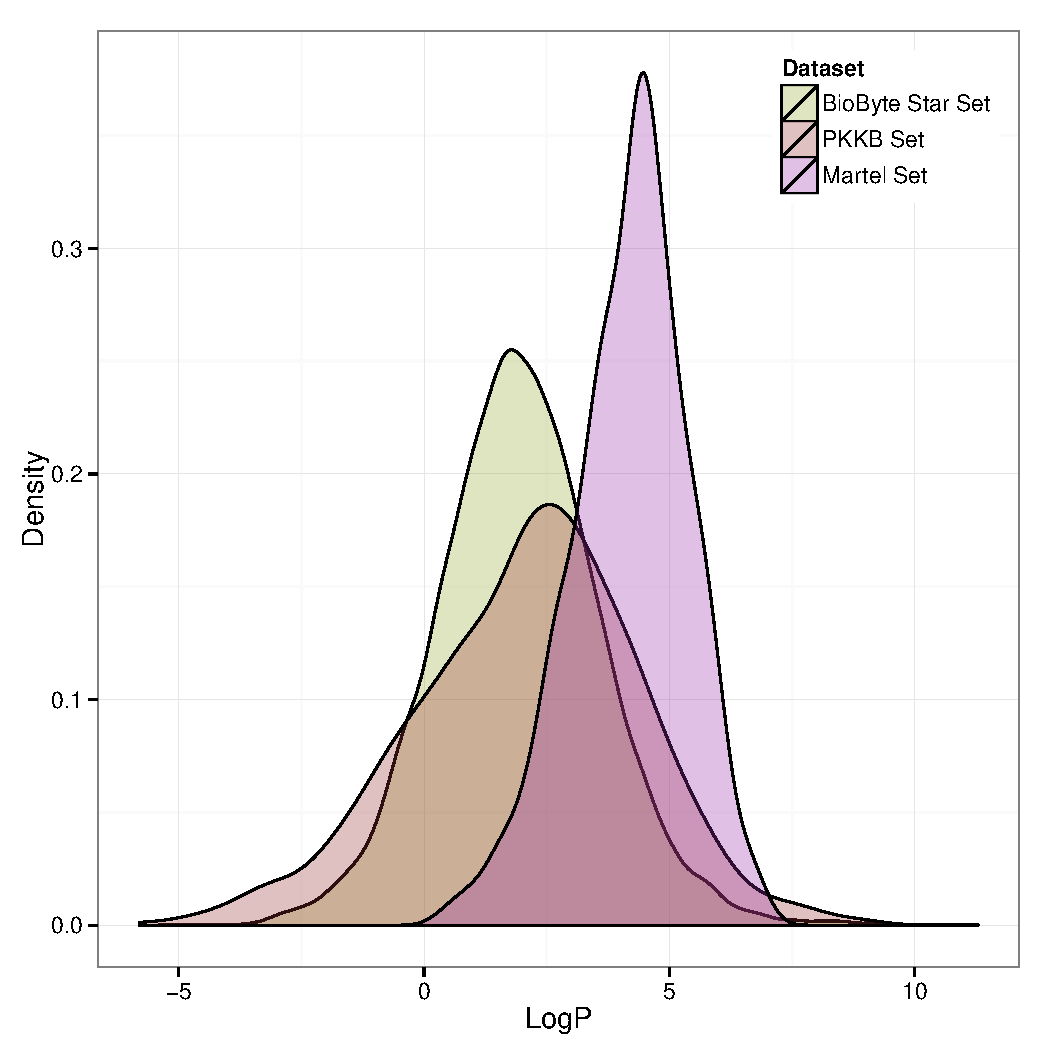
\includegraphics[width=0.9\textwidth]{./Figures/logP_distributions.pdf}
  \caption{Comparison of the distribution of measuered logP values in the training and external test sets.}
  \label{fig:distribution_comparison}
\end{figure}

\begin{figure}[ht]
  \centering
  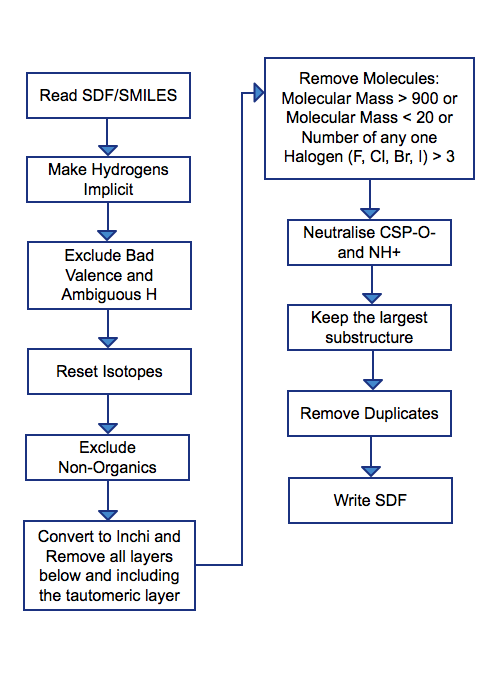
\includegraphics[width=0.5\textwidth]{./Figures/standardisation_workflow.png}
  \caption{The sequence of standardisation and filtering steps undertaken to ensure that molecules presented to the training algorithms were represented similarly.}
  \label{fig:standardisation_workflow}  
\end{figure}

\begin{figure}[ht]
  \centering
  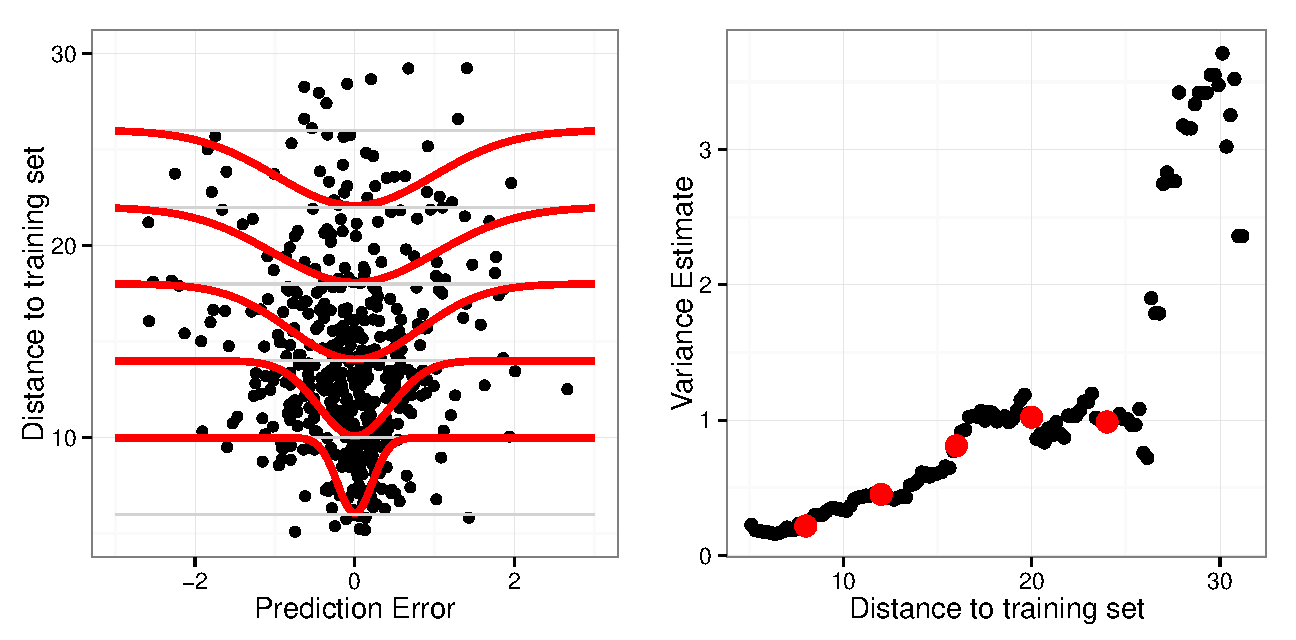
\includegraphics[width=0.9\textwidth]{./Figures/methods_error_estimation.pdf}
  \caption{A visual example of how the variances are estimated from the error in predictions for molecules within a given fixed window in the distance dimension. In this example $P=0$ and $N=1$. Left: Variances are estimated for windows of width 4 with centers 8, 12, 16, 20 and 24. Right: Black points are variances generated considering windows centered at each molecule's distance from the training set. Red points are show where the Gaussian distributions fitted on the left appear when plotting the variance as a function of distance to the training set.}
  \label{fig:methods_error_estimation}
\end{figure} 

\begin{figure}[ht]
  \centering
  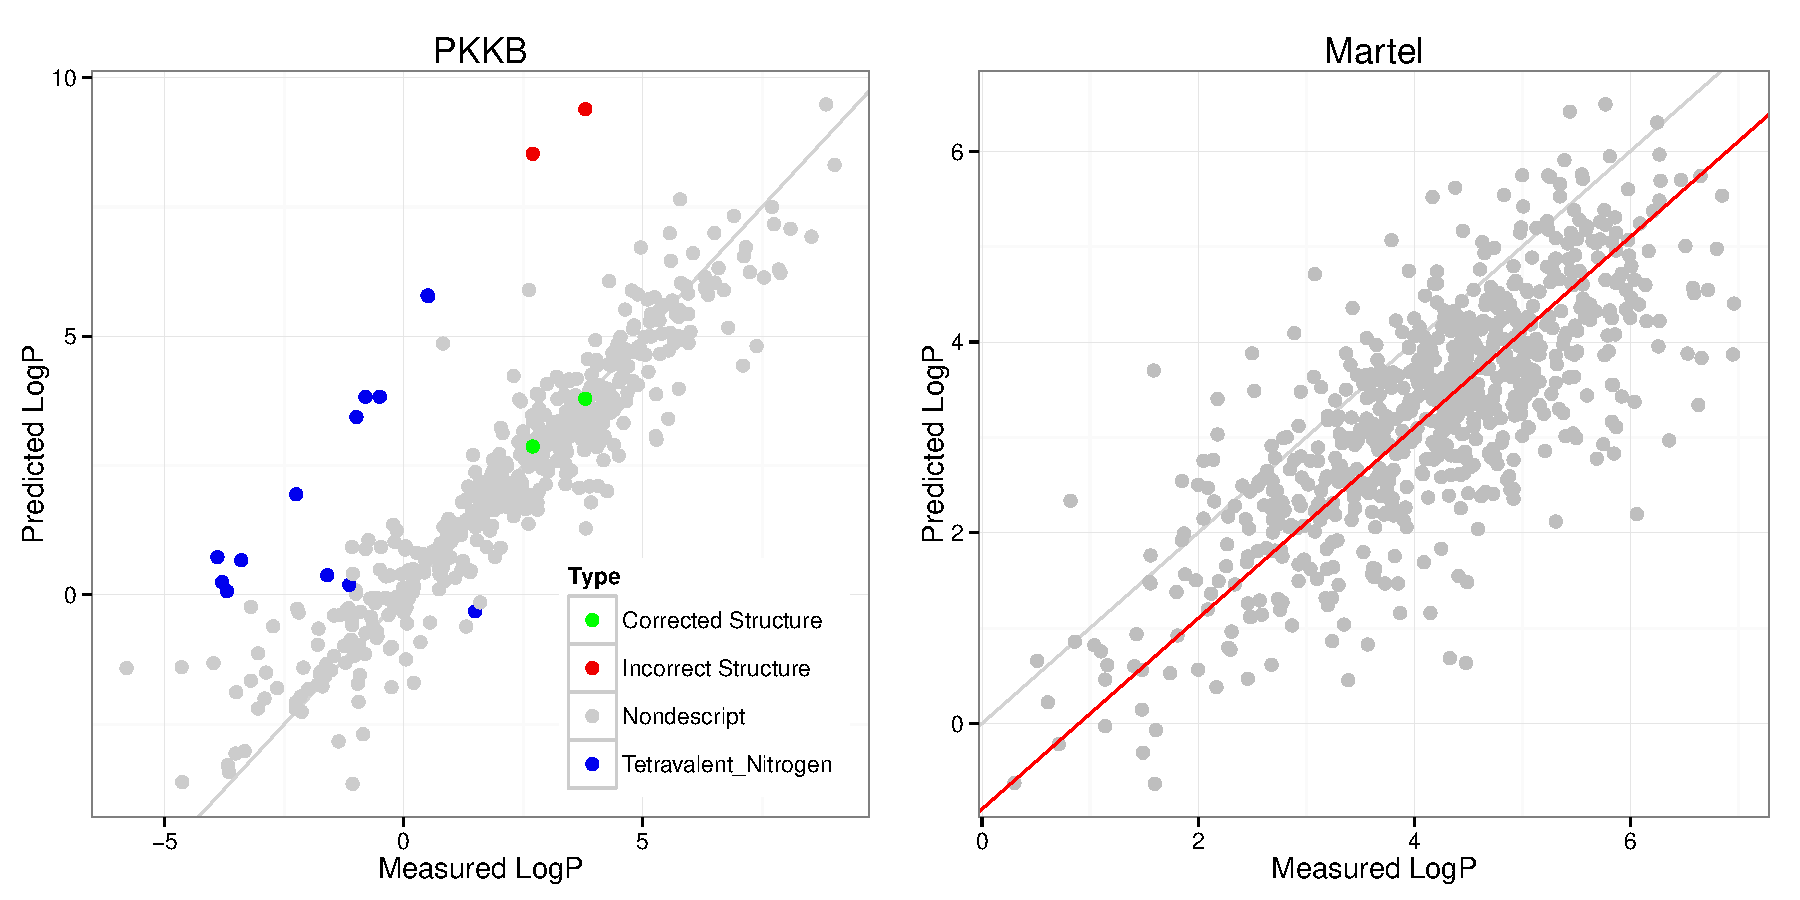
\includegraphics[width=0.9\textwidth]{./Figures/error_analysis_both.pdf}
  \caption{Correlation plots showing the error in predictions on the PKKB and Martel external test sets. In the PKKB set: the logP of the 13 molecules containing tetravalent nitrogens (blue) are, with one exception, overpredicted. The prediction of two molecules in the dataset with incorrect structure (red) is corrected when the correct structures are used (green). Predictions of lower values of logP (below -2.5) are more prone to error. In the Martel set: smLogP underpredicts the set as a whole. The red line is constrained to have slope 1 and is fitted to the data resulting in a y-intercept of -0.897.}
  \label{fig:error_analysis_both}
\end{figure}  

\begin{figure}[ht]
  \centering
  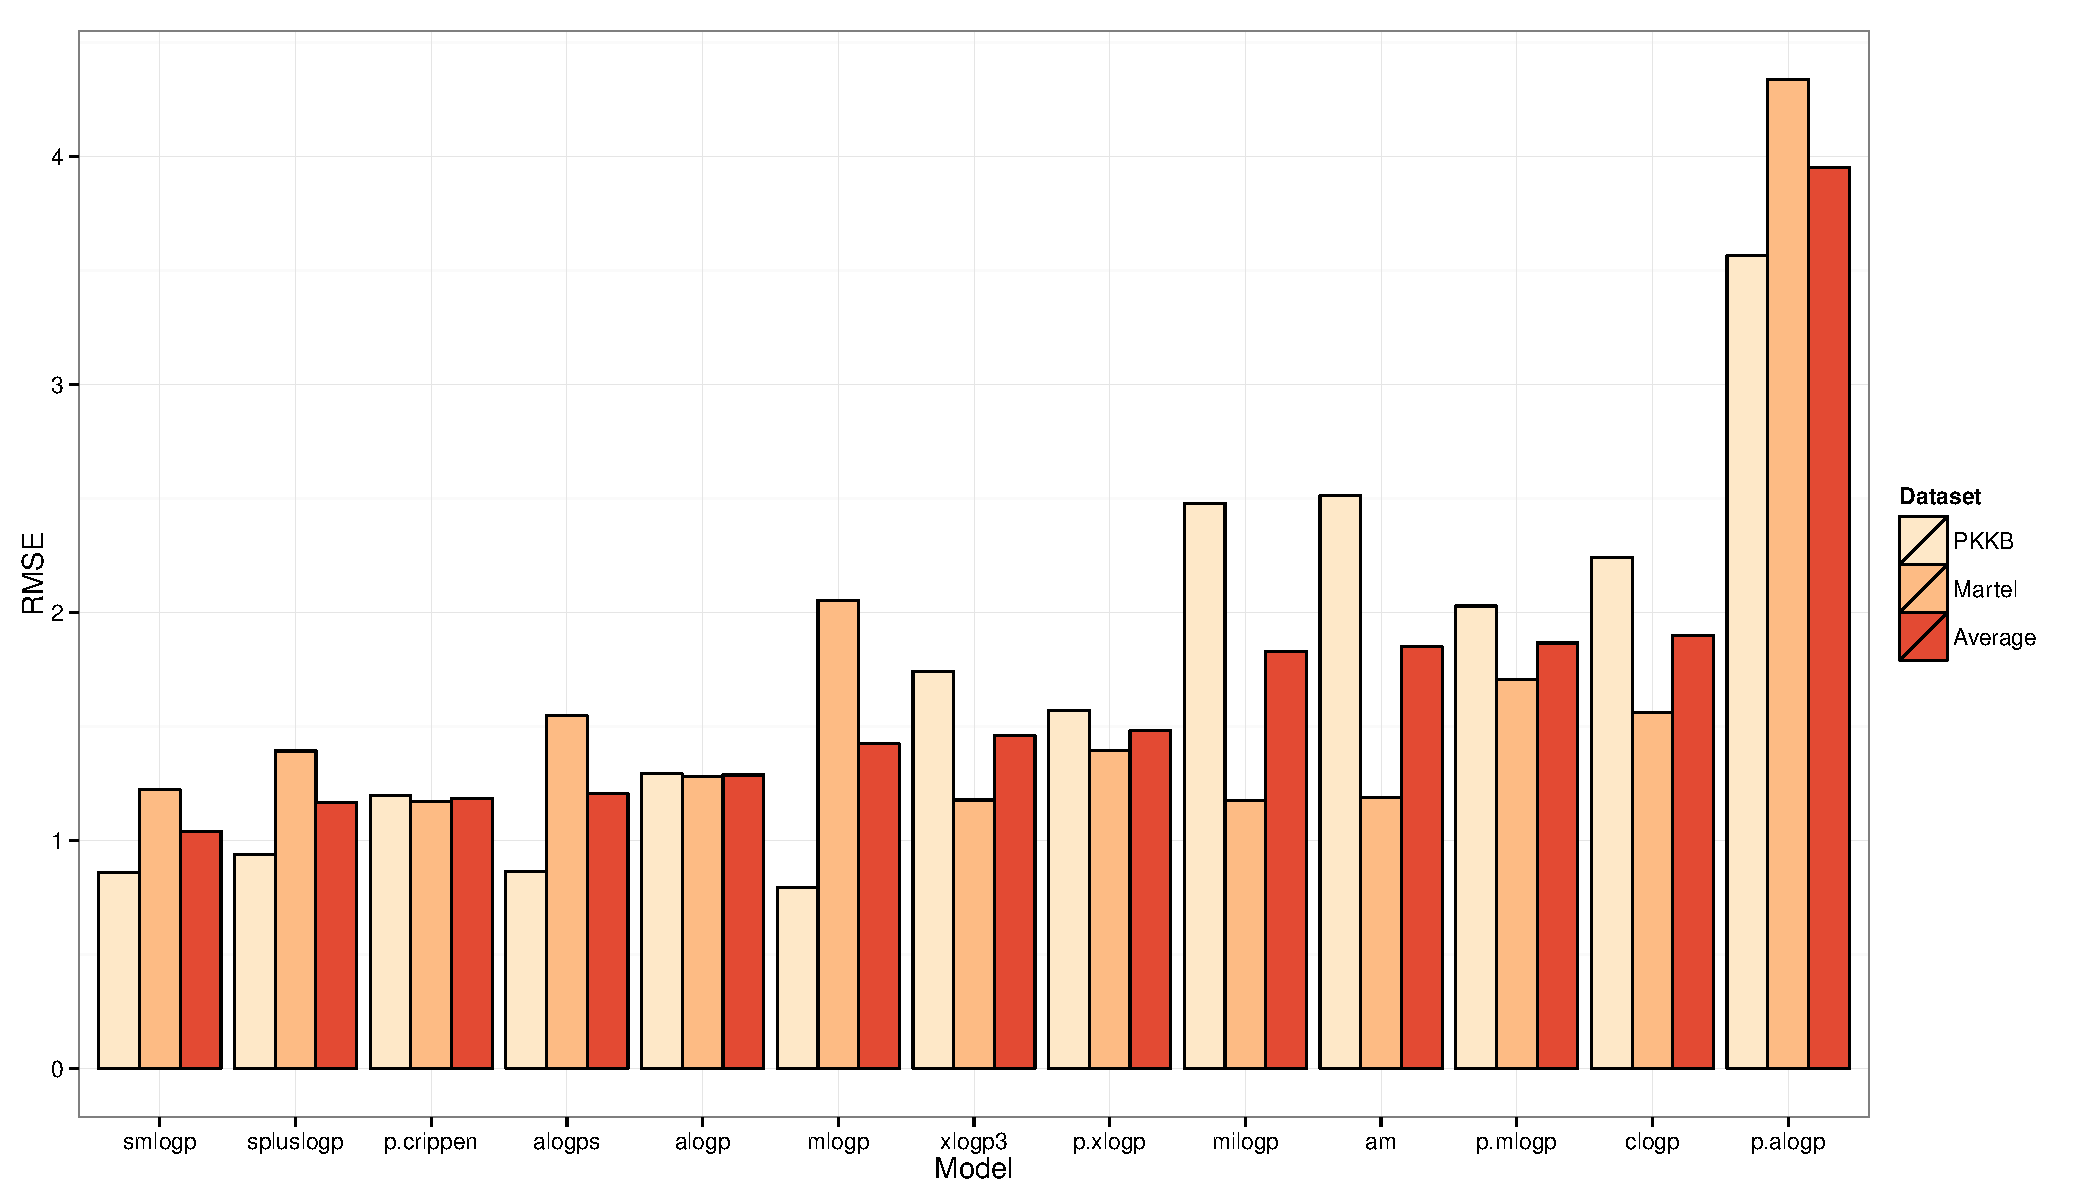
\includegraphics[width=0.9\textwidth]{./Figures/comparison.pdf}
  \caption{Methods are compared by their RMSE on the two external test sets. The methods are placed in ascending order from left to right by the average RMSE over both external test sets. This weights the external test sets equally in the comparison as they contain an unequal number of molecules. Methods prepended by 'p.' are implementations of the PaDEL-Descriptor package. The \textit{am} entry is a baseline model that gives a prediction equal to the mean measured logP value in a particular set for all molecules.}
  \label{fig:comparison}
\end{figure}  

\begin{figure}[ht]
  \centering
  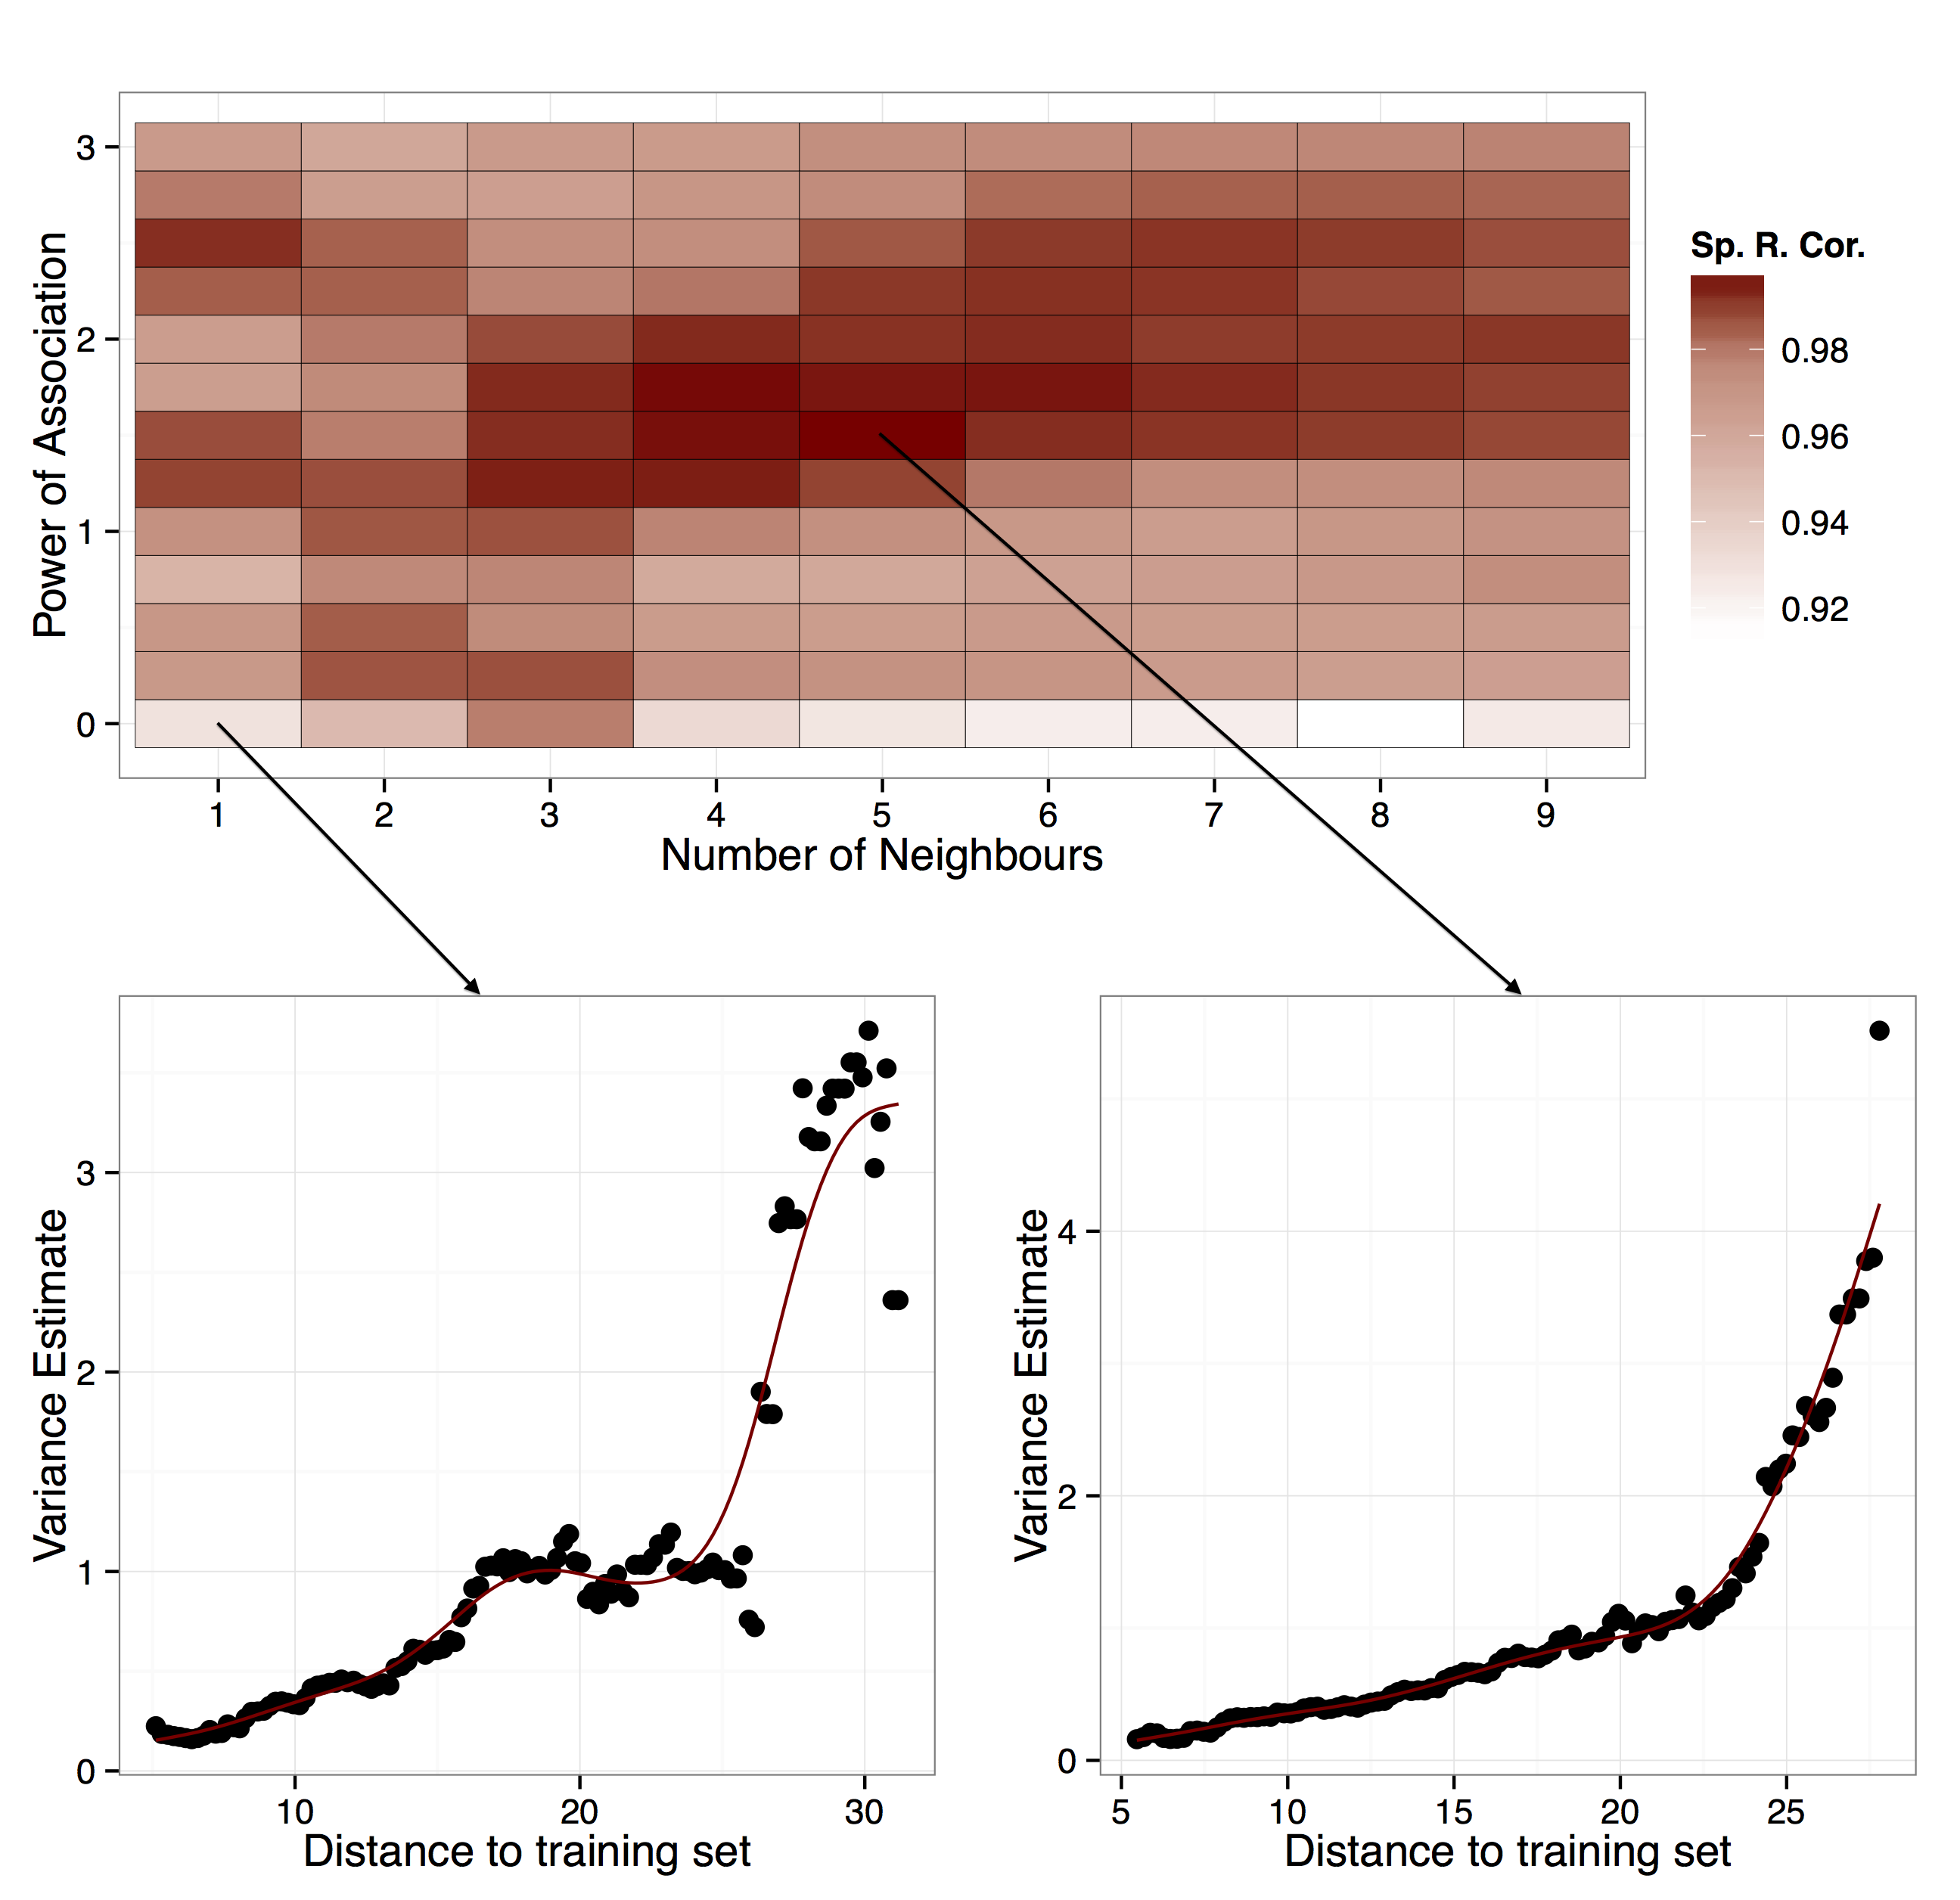
\includegraphics[width=0.9\textwidth]{./Figures/error_estimation.png}
  \caption{Top: Heatmap of Spearman rank correlations of $\tensor{D}{_e^N^P}$ vs $\sigma^2$. Bottom left: $\tensor{D}{_e^N^P}$ vs $\sigma^2$ when $P=0$ and $N=1$. This is what might be naively used when finding a distance to the training set. The spline does not fit this relationship well. Bottom right: $\tensor{D}{_e^N^P}$ vs $\sigma^2$ when $P=1.5$ and $N=5$. This combination of parameters is the maximum rank correlation and falls within a dense region of high rank correlations. The spline fits this relationship much more tightly, leading to more accurate estimation of the variance in the prediction of a new molecule given a distance, $\tensor{D}{_e^N^P}$, calculated from the training set.}
  \label{fig:error_estimation}
\end{figure}

\begin{figure}[ht]
  \centering
  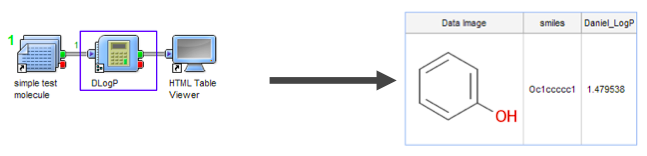
\includegraphics[width=0.9\textwidth]{./Figures/PLP_workflow.png}
  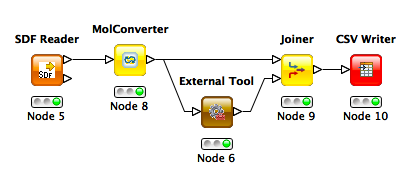
\includegraphics[width=0.9\textwidth]{./Figures/KNIME_workflow.png}
  \caption{Top: Pipeline pilot workflow. Prediction can be incorporated into a single new node. Bottom: Prediction in KNIME is done through a pre-existing external tool node.}
  \label{fig:PLP}
\end{figure}

\end{bmcformat}
\end{document}

% THINGS LEFT TO SAY
% say something about MLOGP from pipeline pilot being different from the one in PaDEL
% include scatter plots of the performance of all models in the SI
% run A to compare the method predictions and see which are most different from each other
% TBD maybe reference literature where the mean skews the predition
% say that the crippen method is most reliable from the padel prediction package
% make a figure that shows the scatter plots of all the methods against the two external data sets
